\documentclass[12pt,letterpaper]{article}
\usepackage{graphicx,textcomp}
\usepackage{natbib}
\usepackage{setspace}
\usepackage{fullpage}
\usepackage{color}
\usepackage[reqno]{amsmath}
\usepackage{amsthm}
\usepackage{fancyvrb}
\usepackage{amssymb,enumerate}
\usepackage[all]{xy}
\usepackage{endnotes}
\usepackage{lscape}
\newtheorem{com}{Comment}
\usepackage{float}
\usepackage{hyperref}
\newtheorem{lem} {Lemma}
\newtheorem{prop}{Proposition}
\newtheorem{thm}{Theorem}
\newtheorem{defn}{Definition}
\newtheorem{cor}{Corollary}
\newtheorem{obs}{Observation}
\usepackage[compact]{titlesec}
\usepackage{dcolumn}
\usepackage{tikz}
\usetikzlibrary{arrows}
\usepackage{multirow}
\usepackage{xcolor}
\newcolumntype{.}{D{.}{.}{-1}}
\newcolumntype{d}[1]{D{.}{.}{#1}}
\definecolor{light-gray}{gray}{0.65}
\usepackage{url}
\usepackage{listings}
\usepackage{color}

\definecolor{codegreen}{rgb}{0,0.6,0}
\definecolor{codegray}{rgb}{0.5,0.5,0.5}
\definecolor{codepurple}{rgb}{0.58,0,0.82}
\definecolor{backcolour}{rgb}{0.95,0.95,0.92}

\lstdefinestyle{mystyle}{
	backgroundcolor=\color{backcolour},   
	commentstyle=\color{codegreen},
	keywordstyle=\color{magenta},
	numberstyle=\tiny\color{codegray},
	stringstyle=\color{codepurple},
	basicstyle=\footnotesize,
	breakatwhitespace=false,         
	breaklines=true,                 
	captionpos=b,                    
	keepspaces=true,                 
	numbers=left,                    
	numbersep=5pt,                  
	showspaces=false,                
	showstringspaces=false,
	showtabs=false,                  
	tabsize=2
}
\lstset{style=mystyle}
\newcommand{\Sref}[1]{Section~\ref{#1}}
\newtheorem{hyp}{Hypothesis}

\title{Problem Set 3/}
\date{Zengyuan Zhao / zhaoze@tcd.ie}
\author{Quant Methods 1/Due: November 11, 2024}


\begin{document}
	\maketitle
	\section*{Instructions}
	\begin{itemize}
		\item Please show your work! You may lose points by simply writing in the answer. If the problem requires you to execute commands in \texttt{R}, please include the code you used to get your answers. Please also include the \texttt{.R} file that contains your code. If you are not sure if work needs to be shown for a particular problem, please ask.
	\item Your homework should be submitted electronically on GitHub.
	\item This problem set is due before 23:59 on Sunday November 11, 2024. No late assignments will be accepted.

	\end{itemize}

		\vspace{.25cm}
	
\noindent In this problem set, you will run several regressions and create an add variable plot (see the lecture slides) in \texttt{R} using the \texttt{incumbents\_subset.csv} dataset. Include all of your code.

	\vspace{.5cm}
\section*{Question 1}
\vspace{.25cm}
\noindent We are interested in knowing how the difference in campaign spending between incumbent and challenger affects the incumbent's vote share. 
	\begin{enumerate}
		\item Run a regression where the outcome variable is \texttt{voteshare} and the explanatory variable is \texttt{difflog}.	\vspace{1cm}
		\lstinputlisting[language=R, firstline=1, lastline=10]{PS03_answersZYZ.R}
		\begin{figure}[h!]
			\caption{\footnotesize{Regression Model of Voteshare and Difflog}}
			\vspace{.5cm}
			\centering
			\label{fig:1.1}
			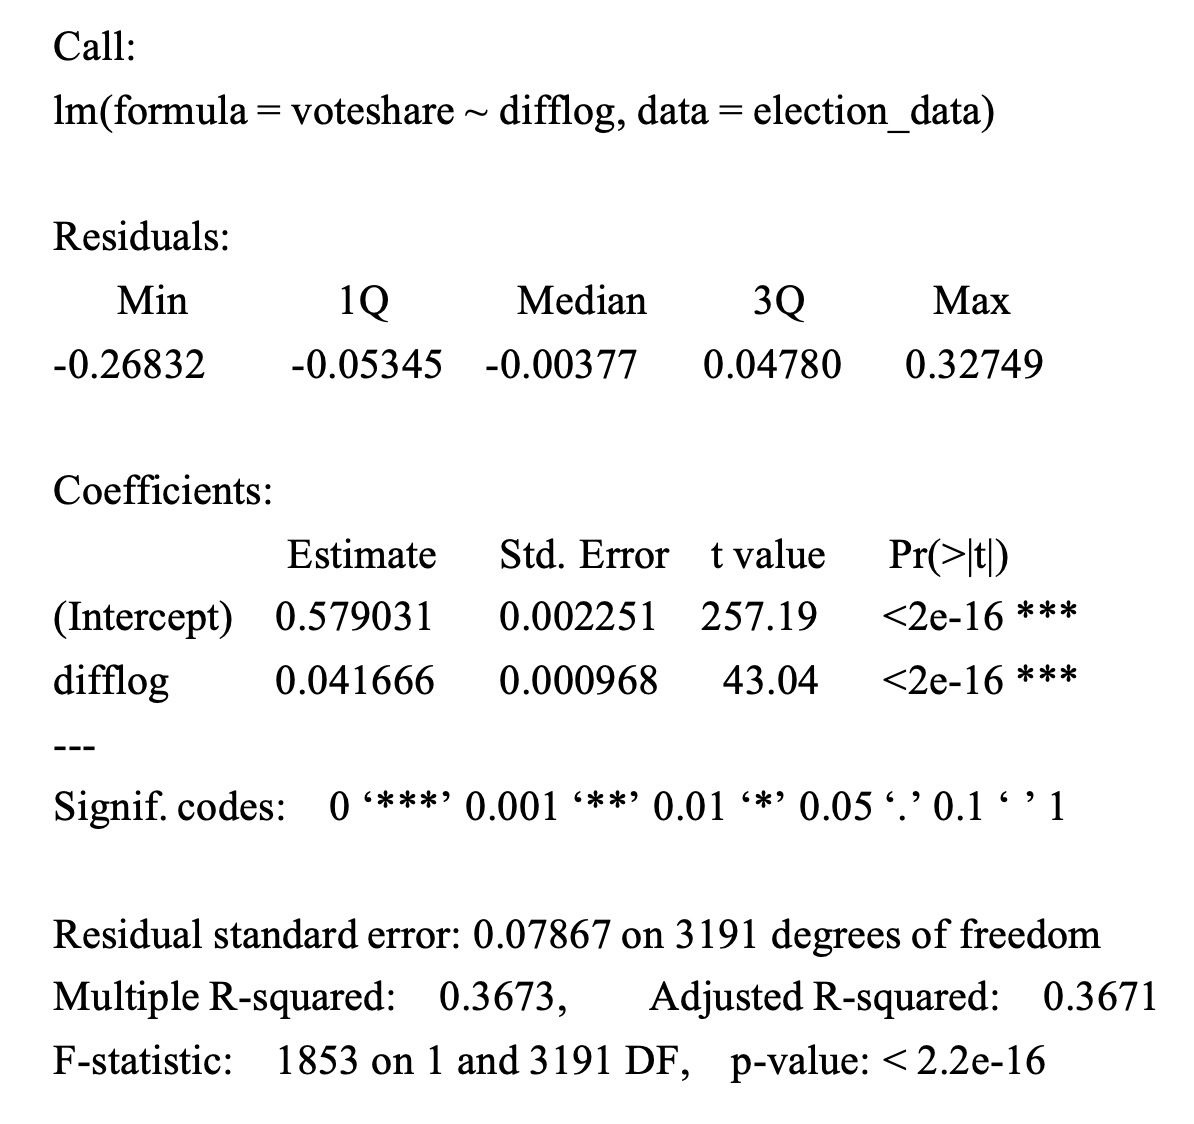
\includegraphics[width=0.7\textwidth]{summary1.png}
		\end{figure}
		
		This regression model explores the impact of the predictor variable difflog on the response variable voteshare. The intercept is estimated at 0.579031, representing the baseline prediction for voteshare when difflog is 0. The coefficient for difflog is 0.041666, which is statistically significant (p-value = 2e-16). This indicates a positive relationship between difflog and voteshare, with an average increase of approximately 0.0417 units in voteshare for each unit increase in difflog.\\
		The coefficient of determination (R-squared) is 0.3673, indicating that difflog explains 36.73 of the total variation in voteshare. The adjusted R-squared is 0.3671, confirming the model's fit after accounting for the number of parameters. The F-statistic is 1853, with a corresponding p-value less than 2.2e-16, demonstrating the statistical significance of the model overall.\\
		
		\item Make a scatterplot of the two variables and add the regression line. 
		\lstinputlisting[language=R, firstline=11, lastline=22]{PS03_answersZYZ.R}
		\begin{figure}[h!]
			\caption{\footnotesize{The Scatter Plot between Voteshare and Difflog}}
			\vspace{.5cm}
			\centering
			\label{fig:1.2}
			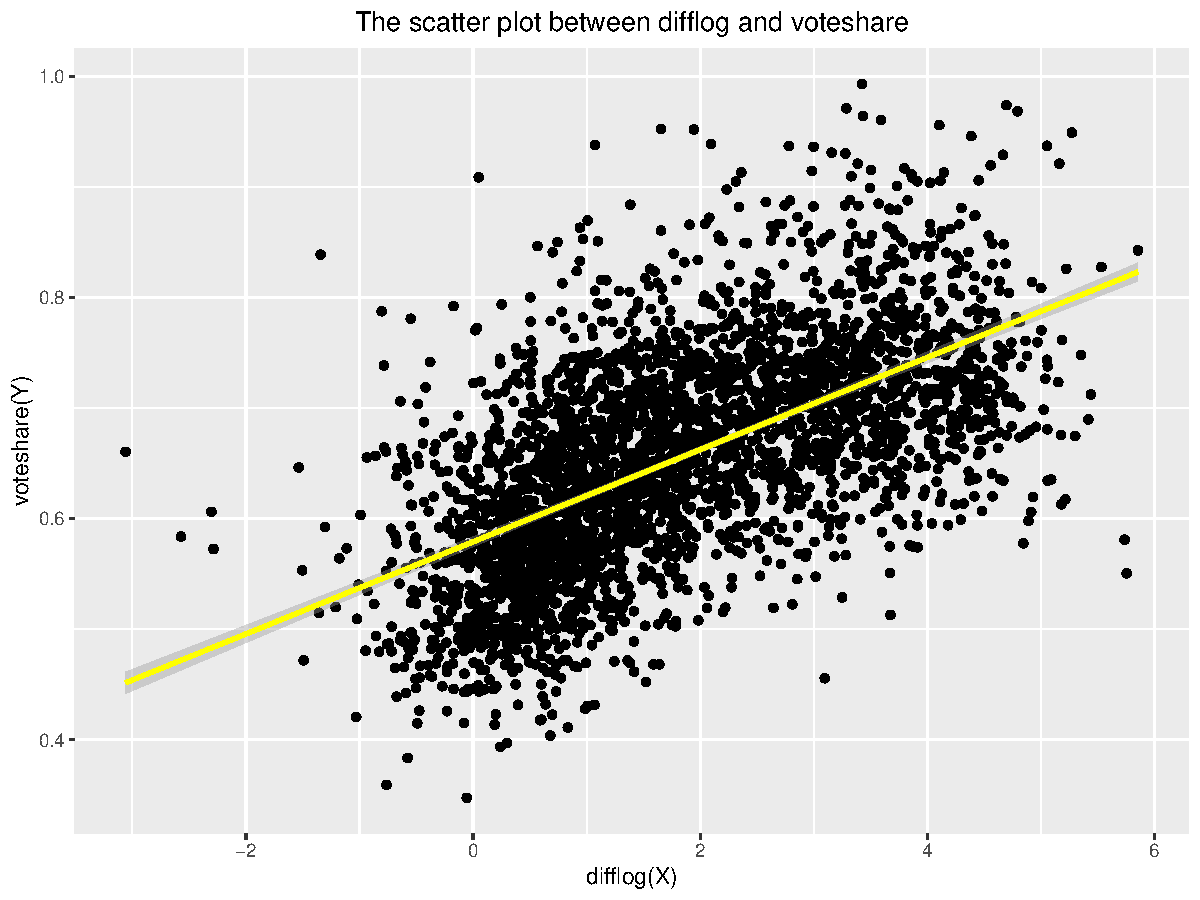
\includegraphics[width=0.7\textwidth]{difflog_voteshare_scatterplot.pdf}
		\end{figure}
		
		This scatterplot reveals the underlying relationship between the variables difflog, which represents the logarithmic difference in expenditures between candidates, and voteshare, which is the share of votes a candidate received. The distribution characteristics of the data points in the figure are significant, mainly concentrated in the central area, and several discrete points can also be seen scattered in other locations, which may reflect the inherent variability and diversity of the data set.\\
		Through further in-depth analysis combined with the regression line drawn in the figure, we found that there is an overall positive correlation trend between difflog and voteshare, that is, as the candidate’s expenditure increases (expressed in the logarithm form of difflog), its gain The vote share (voteshare) also showed a corresponding growth trend. This finding preliminarily indicates that candidates’ financial investment may have affected their election results to some extent.\\
		
		\item Save the residuals of the model in a separate object.	\vspace{1cm}
		\lstinputlisting[language=R, firstline=22, lastline=25]{PS03_answersZYZ.R}
		The following is a display of some residual values between the variable difflog and the variable voteshare:\\
		\begin{figure}[h!]
			\caption{\footnotesize{Partial Residual Value Display}}
			\vspace{.5cm}
			\centering
			\label{fig:1.3}
			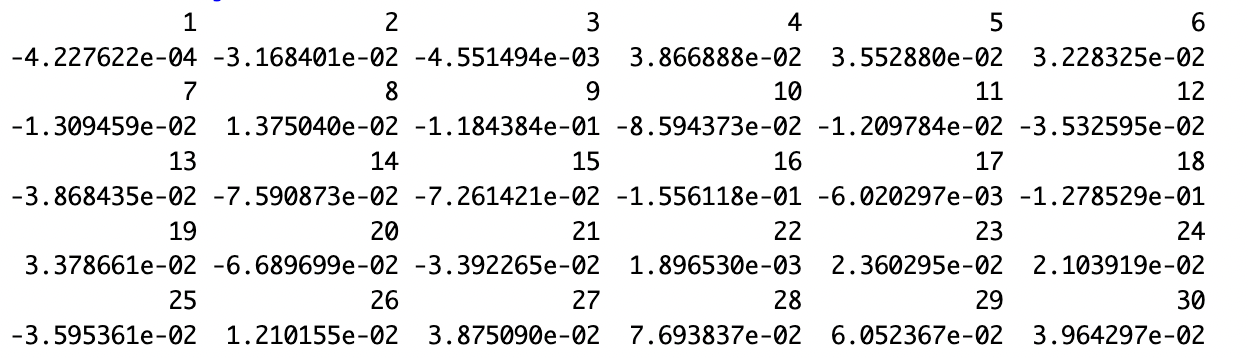
\includegraphics[width=0.8\textwidth]{residuals1.png}
		\end{figure}
		
		\item Write the prediction equation.
		\lstinputlisting[language=R, firstline=26, lastline=30]{PS03_answersZYZ.R}
		"voteshare = 0.579030710920674 + 0.0416663238227399 * difflog"\\
		The formula with three decimal places is:\\
		"voteshare = 0.579 + 0.042 * difflog"\\
	\end{enumerate}
	
\newpage

\section*{Question 2}
\noindent We are interested in knowing how the difference between incumbent and challenger's spending and the vote share of the presidential candidate of the incumbent's party are related.	\vspace{.25cm}
	\begin{enumerate}
		\item Run a regression where the outcome variable is \texttt{presvote} and the explanatory variable is \texttt{difflog}.	\vspace{1cm}
		\lstinputlisting[language=R, firstline=31, lastline=35]{PS03_answersZYZ.R}
		\begin{figure}[h!]
			\caption{\footnotesize{Regression Model of Presvote and Difflog}}
			\vspace{.5cm}
			\centering
			\label{fig:2.1}
			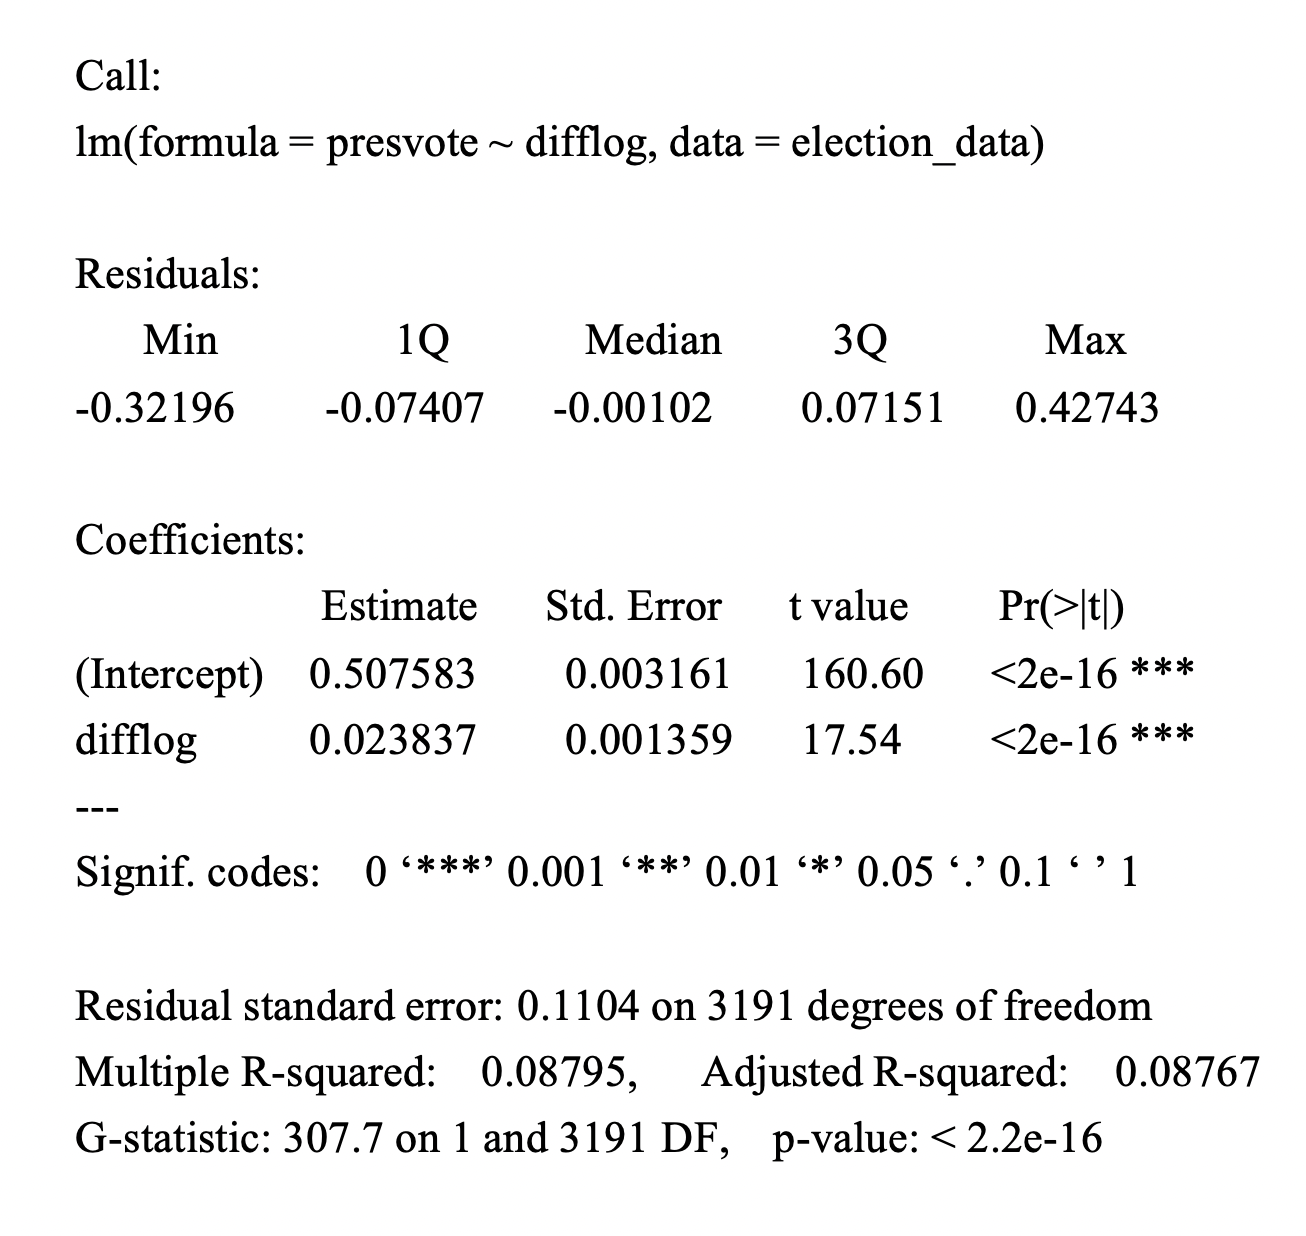
\includegraphics[width=0.7\textwidth]{summary2.png}
		\end{figure}
		
		The model aims to explore the impact of difflog  on presvote. The estimated intercept value is 0.5076, meaning that when difflog is 0, the expected value of presvote is 0.5076. This intercept value is highly significant statistically (p-value < 2e-16), indicating its importance to the model. The coefficient estimate for difflog is 0.0238, suggesting that for every 1-unit increase in difflog, presvote is expected to increase by 0.0238 units. This coefficient is also highly significant statistically (p-value < 2e-16), indicating a significant positive effect of difflog on presvote.\\
		The multiple R-squared value is 0.08795, and the adjusted R-squared value is 0.08767. This suggests that the independent variable in the model accounts for 8.795 (or 8.767 adjusted) of the variation in presvote. The F-statistic is 307.7, with a corresponding p-value less than 2.2e-16. This further confirms that at least one independent variable in the model  has a significant effect on presvote.\\
		
		\item Make a scatterplot of the two variables and add the regression line. 	\vspace{1cm}
		\lstinputlisting[language=R, firstline=36, lastline=46]{PS03_answersZYZ.R}
		\begin{figure}[h!]
			\caption{\footnotesize{The Scatter Plot between Presvote and Difflog}}
			\vspace{.5cm}
			\centering
			\label{fig:2.2}
			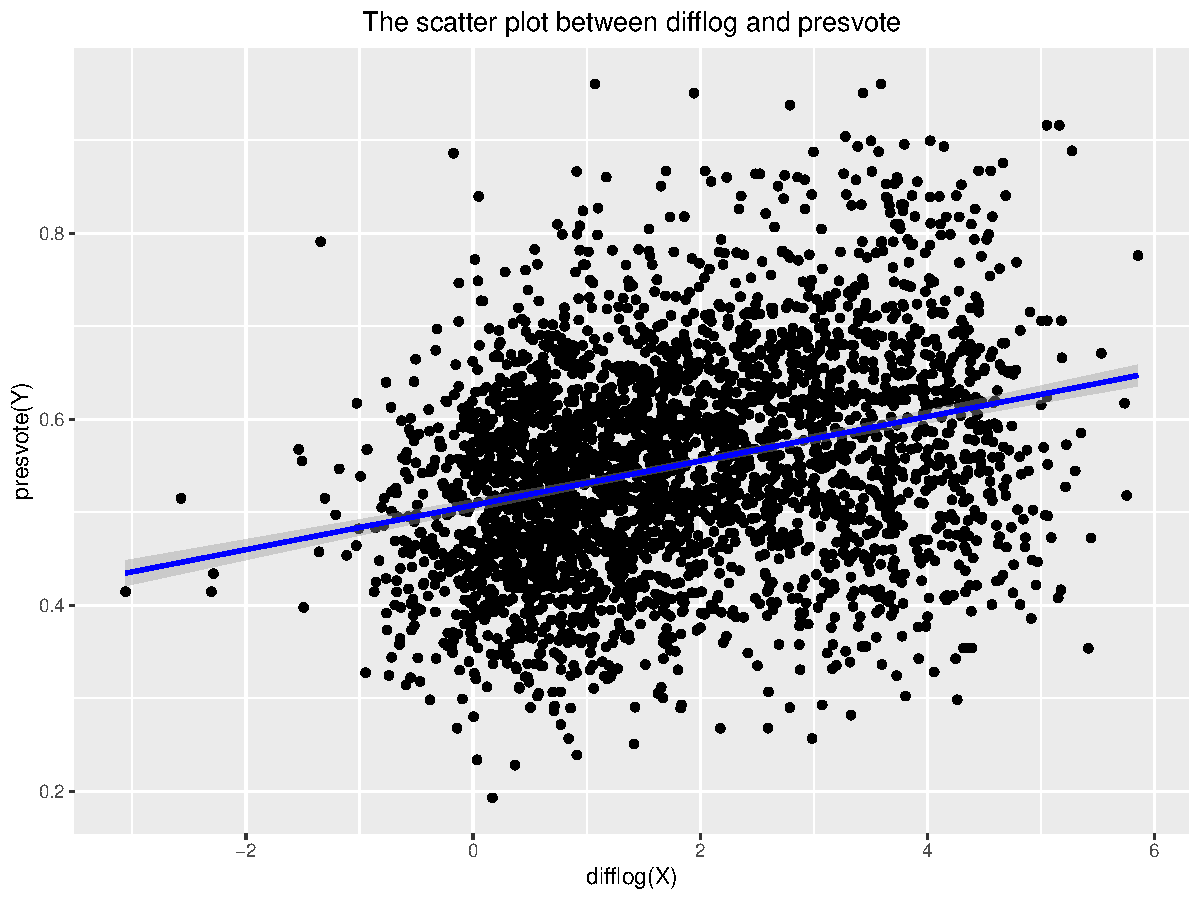
\includegraphics[width=0.7\textwidth]{difflog_presvote_scatterplot.pdf}
		\end{figure}
		\vspace{9cm}
		This scatter plot reveals the underlying relationship between the variables difflog and presvote. The distribution characteristics of the data points in the figure are significant, mainly concentrated in the central area, and several discrete points can also be seen scattered at other locations, which may reflect the inherent variability and diversity of the data set.\\
		Through further in-depth analysis combined with the regression line drawn in the figure, we found that there is an overall positive correlation trend between difflog and presvote, that is, as candidate spending increases (expressed in the logarithm of difflog), the number of presidential candidates of the party where the current president belongs People’s vote share (presvote) also shows a corresponding growth trend. This finding provides preliminary evidence that candidates’ financial commitments may play a role in their electoral outcomes.\\
		
		\item Save the residuals of the model in a separate object.	\vspace{1cm}
		\lstinputlisting[language=R, firstline=47, lastline=49]{PS03_answersZYZ.R}
		The following is a display of some residual values between the variable difflog and the variable presvote:\\
		
		\begin{figure}[h!]
			\caption{\footnotesize{Partial Residual Value Display}}
			\vspace{.5cm}
			\centering
			\label{fig:2.3}
			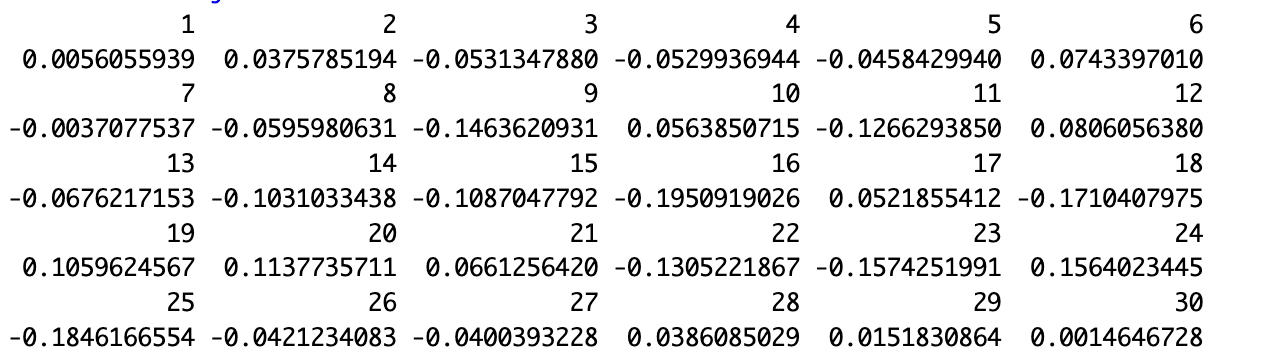
\includegraphics[width=0.8\textwidth]{residuals2.png}
		\end{figure}
		\item Write the prediction equation.
		\lstinputlisting[language=R, firstline=50, lastline=54]{PS03_answersZYZ.R}
		"presvote = 0.507583328405015 + 0.023837233841334 * difflog"\\
		The formula with three decimal places is:\\
		"presvote = 0.508 + 0.024 * difflog"\\
	\end{enumerate}
	
	\newpage	
\section*{Question 3}

\noindent We are interested in knowing how the vote share of the presidential candidate of the incumbent's party is associated with the incumbent's electoral success.
	\vspace{.25cm}
	\begin{enumerate}
		\item Run a regression where the outcome variable is \texttt{voteshare} and the explanatory variable is \texttt{presvote}.
			\vspace{1cm}
		\lstinputlisting[language=R, firstline=55, lastline=59]{PS03_answersZYZ.R}
		
		\begin{figure}[h!]
			\caption{\footnotesize{Regression Model of Presvote and Voteshare}}
			\vspace{.5cm}
			\centering
			\label{fig:3.1}
			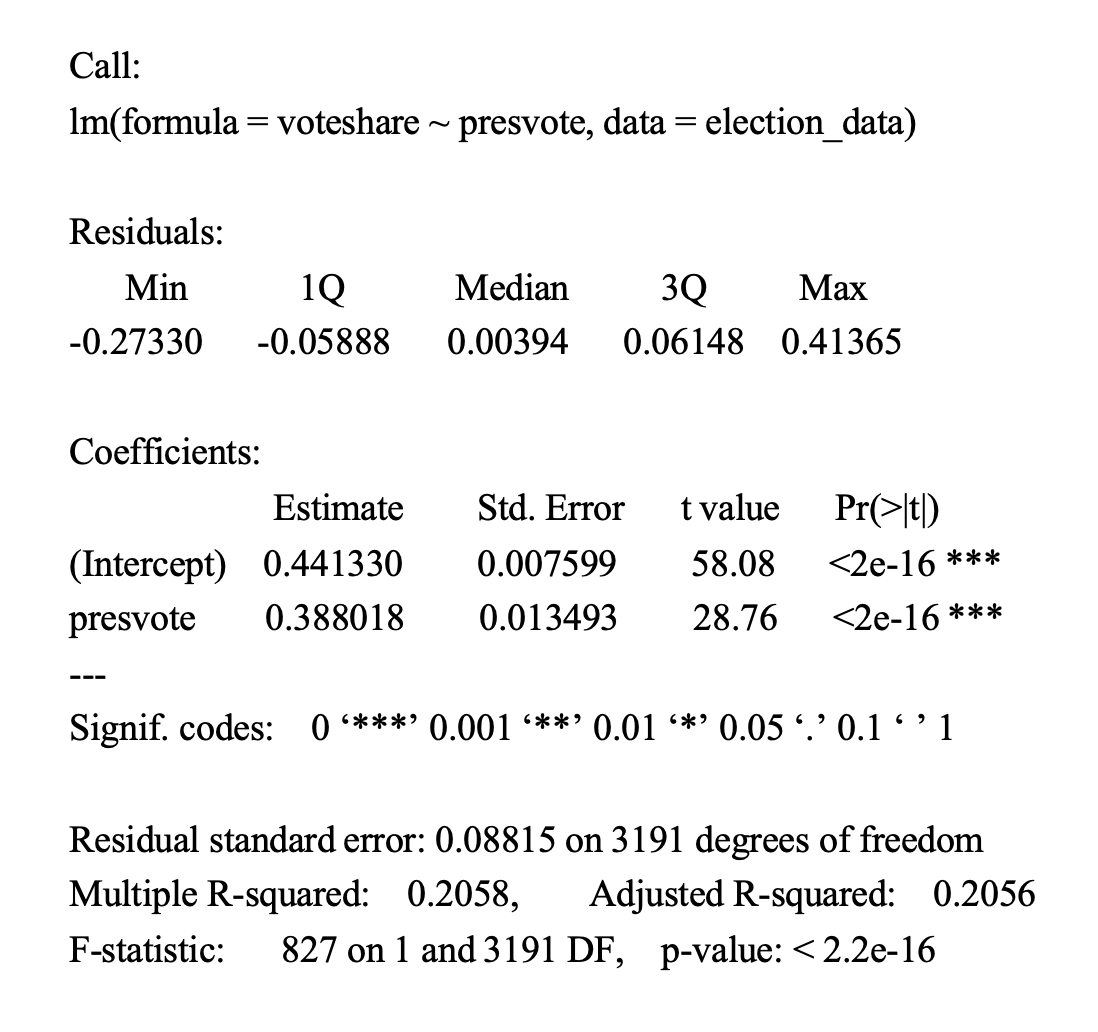
\includegraphics[width=0.7\textwidth]{summary3.png}
		\end{figure}
		
This model explores the impact of the independent variable presvote on the dependent variable voteshare. The regression results show that the intercept is 0.441330, indicating that when presvote is 0, the expected value of voteshare is 0.441330; the coefficient of presvote is 0.388018, indicating that for every unit increase in presvote, voteshare increases by an average of 0.388018 units. Both coefficients are highly statistically significant (both p-values are less than 2e-16), indicating that presvote has a significant impact on voteshare.\\
		In terms of model fit, the standard error of the residual is 0.08815, indicating that the model prediction error is small; the R square is 0.2058, and the adjusted R square is 0.2056, indicating that presvote can explain approximately 20.58 of the change in voteshare.\\
		
		\item Make a scatterplot of the two variables and add the regression line. 
		\vspace{1cm}
		\lstinputlisting[language=R, firstline=60, lastline=70]{PS03_answersZYZ.R}
		
		\begin{figure}[h!]
			\caption{\footnotesize{The Scatter Plot between Presvote and Voteshare}}
			\vspace{.5cm}
			\centering
			\label{fig:3.2}
			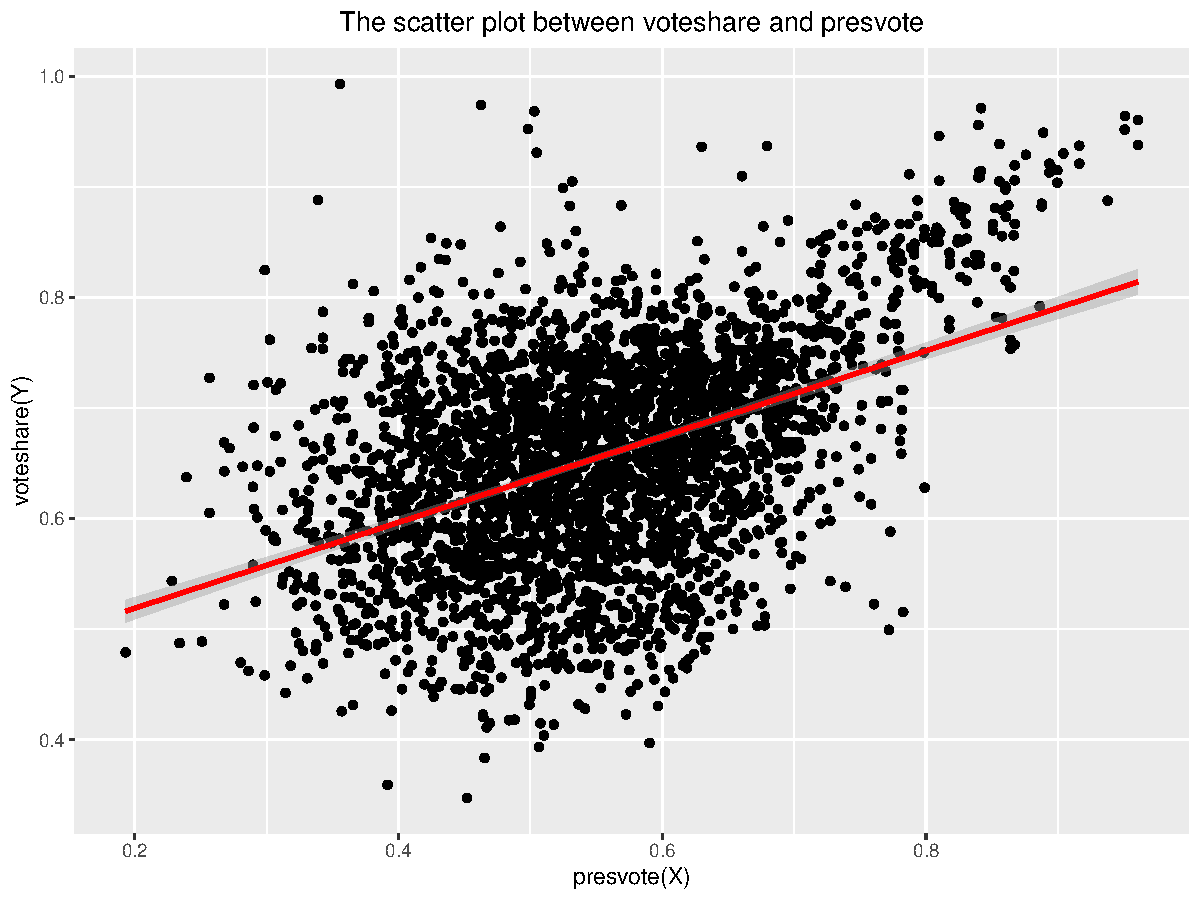
\includegraphics[width=0.6\textwidth]{voteshare_presvote_scatterplot.pdf}
		\end{figure}
		
		    \vspace{5cm}		
		    
		This scatter plot reveals the underlying relationship between the variables presvote and voteshare. The distribution characteristics of the data points in the figure are significant, mainly concentrated in the central area, and several discrete points can also be seen scattered at other locations, which may reflect the inherent variability and diversity of the data set.\\
		Through further in-depth analysis combined with the regression line drawn in the figure, we found that there is an overall positive correlation trend between presvote and voteshare, that is, as the current president’s vote share among the party’s presidential candidates (presvote) increases, the current president’s vote share (voteshare ) is also showing a growing trend.\\

			
		\item Write the prediction equation.
		\lstinputlisting[language=R, firstline=71, lastline=75]{PS03_answersZYZ.R}
		"voteshare = 0.441329881204298 + 0.38801844338744 * presvote"\\
		The formula with three decimal places is:\\
		"voteshare = 0.441 + 0.388 * presvote"\\
	\end{enumerate}
	

\newpage	
\section*{Question 4}
\noindent The residuals from part (a) tell us how much of the variation in \texttt{voteshare} is $not$ explained by the difference in spending between incumbent and challenger. The residuals in part (b) tell us how much of the variation in \texttt{presvote} is $not$ explained by the difference in spending between incumbent and challenger in the district.
	\begin{enumerate}
		\item Run a regression where the outcome variable is the residuals from Question 1 and the explanatory variable is the residuals from Question 2.	\vspace{1cm}
		\lstinputlisting[language=R, firstline=76, lastline=80]{PS03_answersZYZ.R}

	\begin{figure}[h!]
	\caption{\footnotesize{Regression Model of Two Groups of Residuals}}
	\vspace{.5cm}
	\centering
	\label{fig:4.1}
	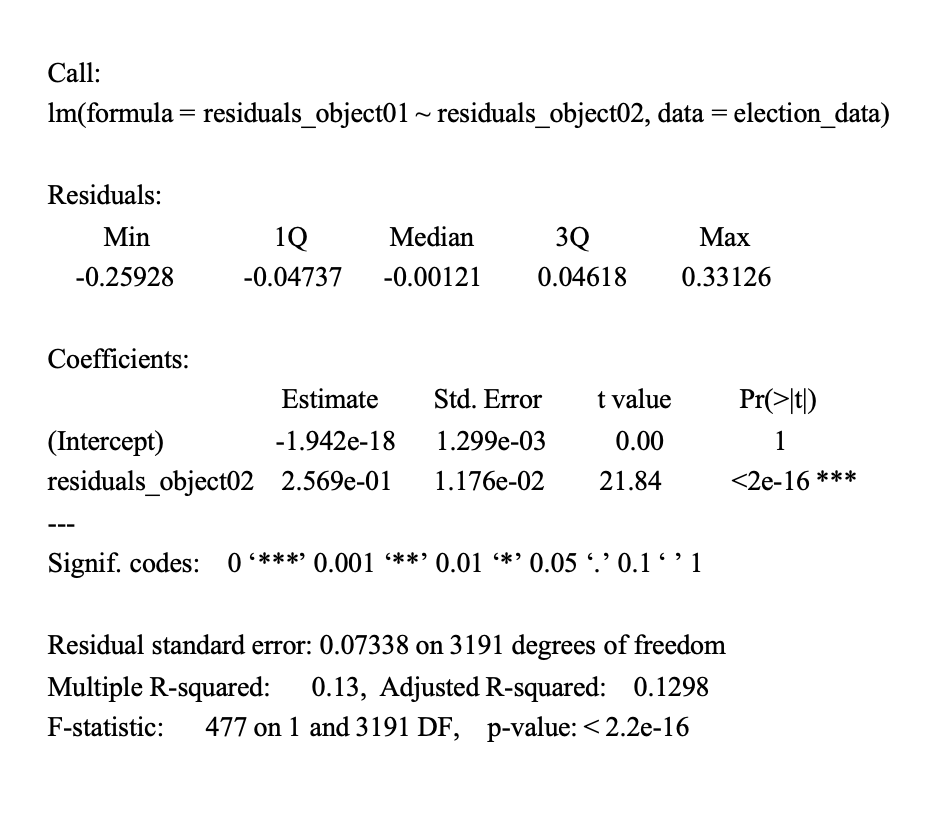
\includegraphics[width=0.7\textwidth]{summary4.png}
	\end{figure}

This model aims to explore the relationship between two sets of residual values. This intercept value is not statistically significant (p-value = 1), indicating that when residuals2 is 0, the expected value of residuals1 does not deviate significantly from 0. The coefficient of residuals2 is 2.569e-01, and the p-value is less than 2e-16. This shows that for every unit increase in residuals2, residuals1 increases by 0.2569 units on average, and this relationship is highly statistically significant. The standard error of the residual is 0.07338, indicating that the error of the model prediction is relatively small.\\
The R square is 0.13 and the adjusted R square is 0.1298, indicating that residuals2 can explain about 13  of the variation of residuals1. F statistic: 477, the corresponding p value is less than 2.2e-16, further confirming that residuals2 has a significant impact on residuals1.\\

		\item Make a scatterplot of the two residuals and add the regression line. 	\vspace{1cm}
		\lstinputlisting[language=R, firstline=81, lastline=91]{PS03_answersZYZ.R}

\begin{figure}[h!]
	\caption{\footnotesize{The Scatter Plot between Two Groups of Residuals}}
	\vspace{.5cm}
	\centering
	\label{fig:4.2}
	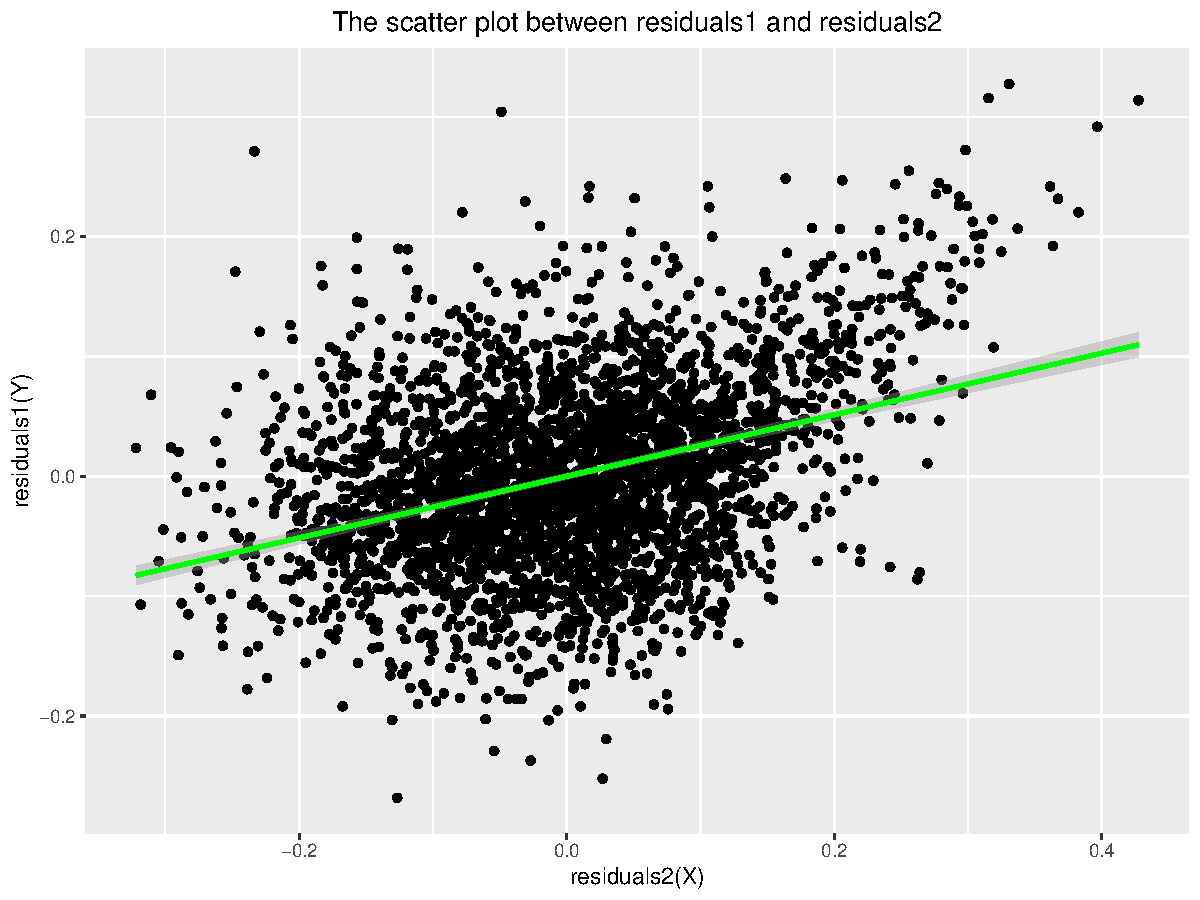
\includegraphics[width=0.6\textwidth]{residuals1_residuals2_scatterplot.pdf}
\end{figure}
	\vspace{5cm}		
	
This scatter plot reveals the underlying relationship between the two sets of residuals. The distribution characteristics of the data points in the figure are significant, mainly concentrated in the central area, and several discrete points can also be seen at other locations, which may reflect the inherent variability and diversity of the data set.\\
Through further in-depth analysis combined with the regression line drawn in the figure, we found that there is an overall positive correlation trend between residuals1 and residuals2.\\

		\item Write the prediction equation.
		\lstinputlisting[language=R, firstline=92, lastline=96]{PS03_answersZYZ.R}
		"residuals1 = -1.94153862344556e-18 + 0.256877012700097 * residuals2"\\
		The formula with three decimal places is:\\
		"residuals1 = -1.94153862344556e-18 + 0.257 * residuals2"\\
	\end{enumerate}
	
	\newpage	

\section*{Question 5}
\noindent What if the incumbent's vote share is affected by both the president's popularity and the difference in spending between incumbent and challenger? 
	\begin{enumerate}
		\item Run a regression where the outcome variable is the incumbent's \texttt{voteshare} and the explanatory variables are \texttt{difflog} and \texttt{presvote}.	
		\lstinputlisting[language=R, firstline=97, lastline=101]{PS03_answersZYZ.R}
		
	\begin{figure}[h!]
			\caption{\footnotesize{Regression Model of Voteshare with Difflog and Presvote}}
			\vspace{.5cm}
			\centering
			\label{fig:5.1}
			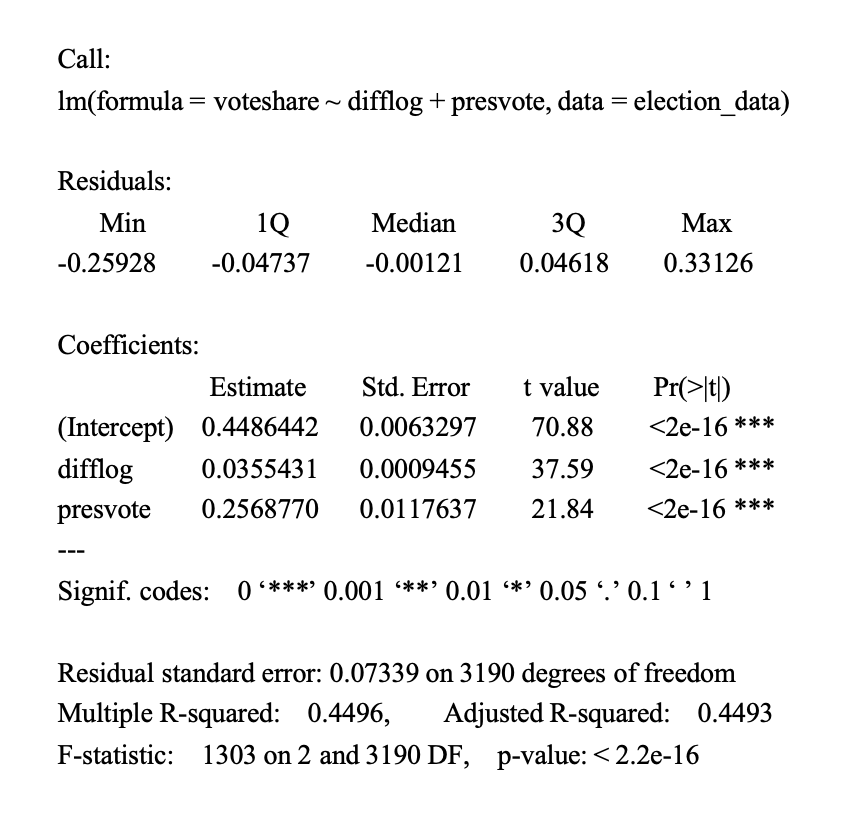
\includegraphics[width=0.7\textwidth]{summary5.png}
	\end{figure}
	\vspace{5cm}		
	This model aims to analyze the relationship between vote share and two explanatory variables difflog and presvote. When difflog and presvote are both 0, the incumbent's expected vote share is 0.4486. This value is highly statistically significant (p < 2e-16), indicating that the intercept contributes significantly to the model. \\
	The coefficient of difflog is estimated to be 0.0355, indicating that while keeping presvote constant, voteshare will increase by 0.0355 units for every unit increase in difflog. This coefficient is also highly statistically significant (p < 2e-16), indicating that spending differences have a significant impact on vote shares.\\
	The coefficient of presvote is estimated to be 0.2569, indicating that while keeping the difflog constant, voteshare will increase by 0.2569 units for every unit increase in presvote. This coefficient is also statistically highly significant (p < 2e-16), indicating that the variable presvote has a significant impact on voteshare.\\
	The R-squared is 0.4496 and the adjusted R-squared is 0.4493, indicating that the number of variables in the model is reasonable. The F-statistic is 1303, and the corresponding p-value is less than 2.2e-16, indicating that the model is significant as a whole, that is, at least one explanatory variable has a significant impact on the dependent variable.\\
	
		\item Write the prediction equation.	\vspace{0.5cm}
		\lstinputlisting[language=R, firstline=102, lastline=106]{PS03_answersZYZ.R}
		"voteshare = 0.448644221823622 + 0.0355430864025444 * difflog + 0.256877012700098 * presvote"\\
		The formula with three decimal places is:\\
		"voteshare = 0.449 + 0.036 * difflog + 0.257 * presvote"\\
		\item What is it in this output that is identical to the output in Question 4? Why do you think this is the case? \vspace{0.5cm}
		\vspace{0.5cm}
		
		After observation, the output of this question has the following characteristics as the output of Question 4:\\
		1. Residual distribution:\\
		The residual minimum (Min), first quartile (1Q), median (Median), third quartile (3Q) and maximum (Max) of the two models are exactly the same. This shows that the residuals of the two models have similar characteristics in distribution, that is, their statistics such as minimum, median and maximum are the same. This may be because both models use the same data set and the errors or variability in the data are similarly reflected in the two models.\\
		2. Similarity of residual standard errors:\\
		The residual standard errors of the two models are very close, 0.07338 and 0.07339 respectively. The two models have similar residual standard errors, which may mean that they have certain similarities in predictive ability, although this similarity may be affected by the model structure and the choice of explanatory variables.\\
		Reason\\
		1. Consistency of data sets: Both models use the same data set , so their data sources and data processing methods are consistent. This may cause the two models to show similarities in residual distribution and residual standard errors.\\
		2. Universality of model evaluation indicators: Residual distribution and residual standard errors are universal, so these indicators may show similarities even if the structure and explanatory variables of the models are different.\\
	\end{enumerate}




\end{document}
